\documentclass[a4paper]{article}
\usepackage{float}
\usepackage[utf8]{inputenc}
\usepackage[T1]{fontenc}
\usepackage{graphicx}
\usepackage[frenchb]{babel}
\usepackage{amsmath}
\usepackage{listings}

% define our color
\usepackage{xcolor}

% code color
\definecolor{ligthyellow}{RGB}{250,247,220}
\definecolor{darkblue}{RGB}{5,10,85}
\definecolor{ligthblue}{RGB}{1,147,128}
\definecolor{darkgreen}{RGB}{8,120,51}
\definecolor{darkred}{RGB}{160,0,0}

% other color
\definecolor{ivi}{RGB}{141,107,185}


\lstset{
    language=scilab,
    captionpos=b,
    extendedchars=true,
    frame=lines,
    numbers=left,
    numberstyle=\tiny,
    numbersep=5pt,
    keepspaces=true,
    breaklines=true,
    showspaces=false,
    showstringspaces=false,
    breakatwhitespace=false,
    stepnumber=1,
    showtabs=false,
    tabsize=3,
    basicstyle=\small\ttfamily,
    backgroundcolor=\color{ligthyellow},
    keywordstyle=\color{ligthblue},
    morekeywords={include, printf, uchar},
    identifierstyle=\color{darkblue},
    commentstyle=\color{darkgreen},
    stringstyle=\color{darkred},
}

\begin{document}

\title{VISA -- TP Couleurs}
\author{Arnaud Cojez}
\date{mercredi 9 novembre 2016}

\maketitle

\newpage
\tableofcontents
\newpage
%----------------------------------------------------------------------------------------
%	INTRODUCTION
%----------------------------------------------------------------------------------------

\section{Introduction}
Une fois la capture de la lumière maîtrisée, il nous faut définir la façon dont sera stockée l'image formée.\\
L'information des pixels d'une image peut être stockée selon différentes représentations. Par exemple, nous pouvons considérer différentes couleurs comme les composantes de l'image.\\
Ainsi, chaque opération effectuée sur une image aura un effet lié à la représentation de celle-ci.\\

Le long de ce TP, nous utiliserons l'espace de couleurs HSB (Hue-Saturation-Brightness). Celui-ci nous permet de modifier la luminance, la teinte et la saturation de l'image.\\
Les fichiers utilisés sont des images composant le test d'Ishihara, qui permet de détecter les déficiences dichromatiques telles que le daltonisme.

\begin{figure}[H]
\begin{center}
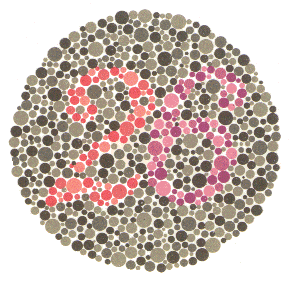
\includegraphics[width=170px]{../base/cas_1_dalton26.png}
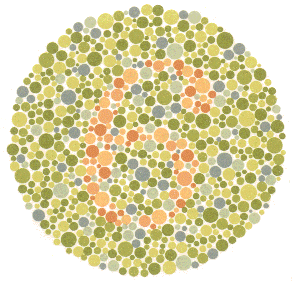
\includegraphics[width=170px]{../base/cas_4_dalton6.png}
\end{center}
\caption{Planches issues du Test d'Ishihara}
\end{figure}


\clearpage
%----------------------------------------------------------------------------------------
%	MANIPULATION DE LA LUMINANCE
%----------------------------------------------------------------------------------------

\section{Manipulation de la luminance}

\subsection{Explication}

TODO expliquer principe

\subsubsection{Cas 1}

\begin{figure}[H]
\begin{center}
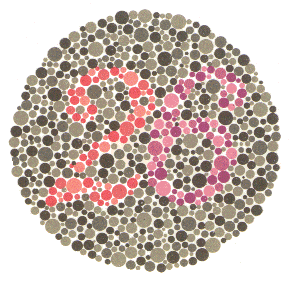
\includegraphics[width=170px]{../base/cas_1_dalton26.png}
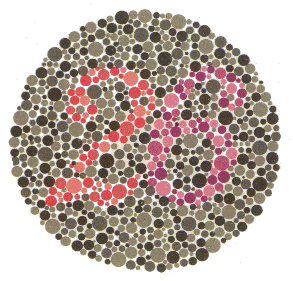
\includegraphics[width=170px]{../base/cas_1_luminance.png}
\end{center}
\caption{À gauche, image originale. À droite, image modifiée}
\end{figure}

\begin{figure}[H]
\begin{center}
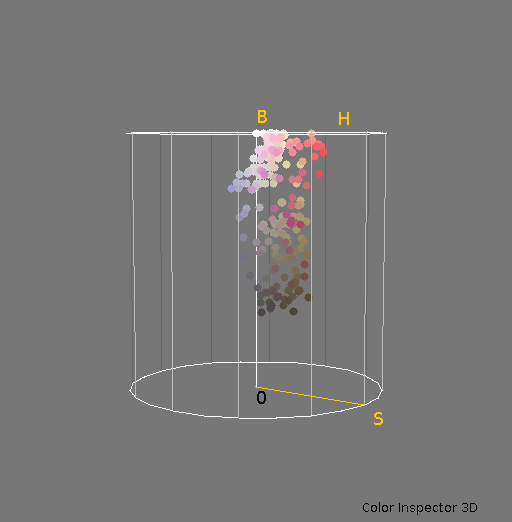
\includegraphics[width=170px]{../resultats/e1_q1_k1_26.png}
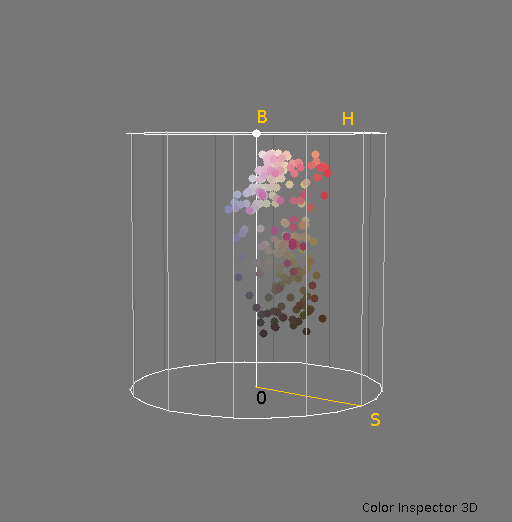
\includegraphics[width=170px]{../resultats/e1_q1_k1_lumi.png}
\end{center}
\caption{Visualisation des 2 images dans l'espace HSB}
\end{figure}

TODO expliquer différence estimée

\clearpage
\subsubsection{Cas 2}

\begin{figure}[H]
\begin{center}
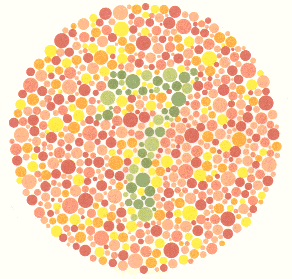
\includegraphics[width=170px]{../base/cas_2_dalton7.png}
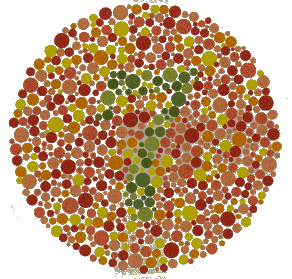
\includegraphics[width=170px]{../base/cas_2_luminance.png}
\end{center}
\caption{À gauche, image originale. À droite, image modifiée}
\end{figure}

\begin{figure}[H]
\begin{center}
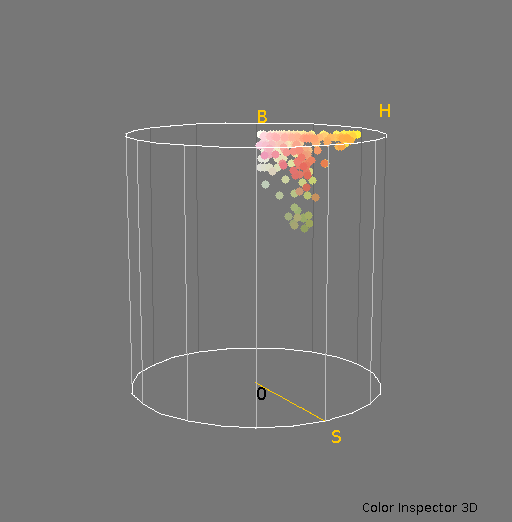
\includegraphics[width=170px]{../resultats/e1_q1_k2_7.png}
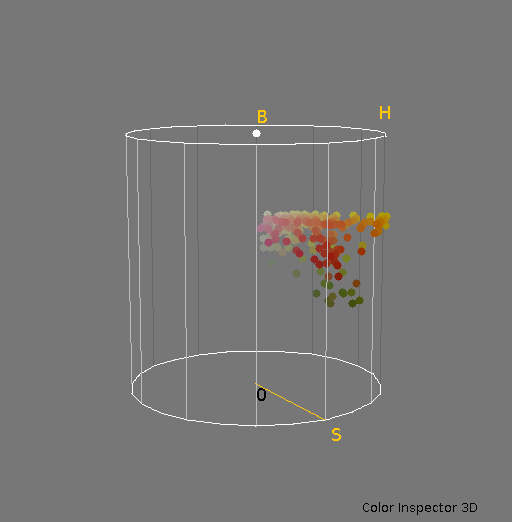
\includegraphics[width=170px]{../resultats/e1_q1_k2_lumi.png}
\end{center}
\caption{Visualisation des 2 images dans l'espace HSB}
\end{figure}

TODO expliquer différence estimée

\clearpage
\subsubsection{Cas 3}

\begin{figure}[H]
\begin{center}
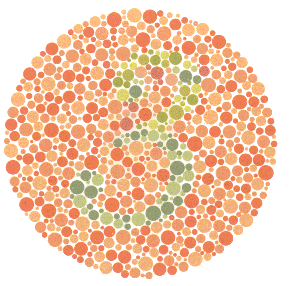
\includegraphics[width=170px]{../base/cas_3_dalton3.png}
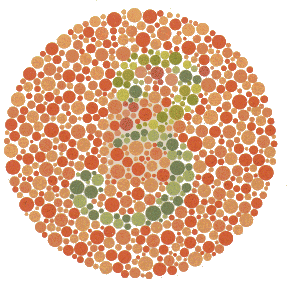
\includegraphics[width=170px]{../base/cas_3_luminance.png}
\end{center}
\caption{À gauche, image originale. À droite, image modifiée}
\end{figure}

\begin{figure}[H]
\begin{center}
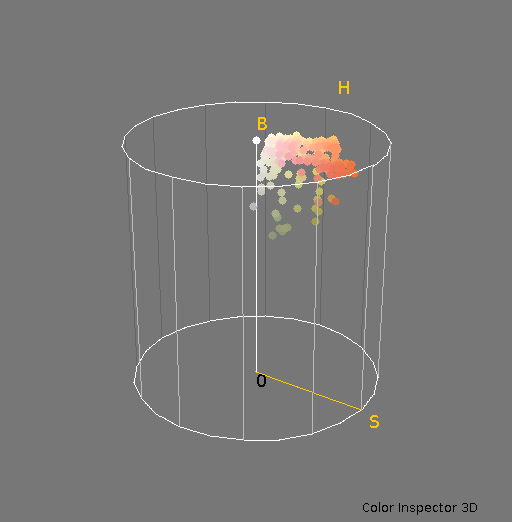
\includegraphics[width=170px]{../resultats/e1_q1_k3_3.png}
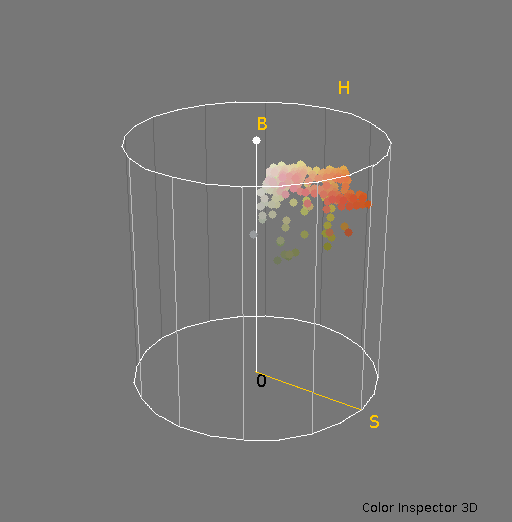
\includegraphics[width=170px]{../resultats/e1_q1_k3_lumi.png}
\end{center}
\caption{Visualisation des 2 images dans l'espace HSB}
\end{figure}

TODO expliquer différence estimée

\clearpage
\subsubsection{Cas 4}

\begin{figure}[H]
\begin{center}
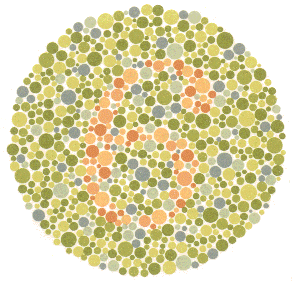
\includegraphics[width=170px]{../base/cas_4_dalton6.png}
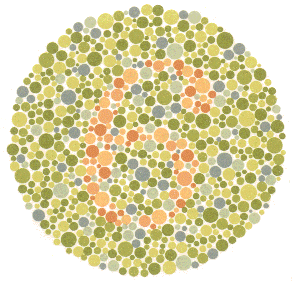
\includegraphics[width=170px]{../base/cas_4_luminance.png}
\end{center}
\caption{À gauche, image originale. À droite, image modifiée}
\end{figure}

\begin{figure}[H]
\begin{center}
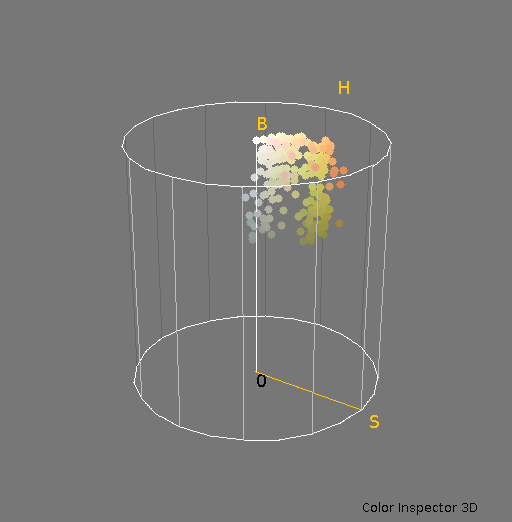
\includegraphics[width=170px]{../resultats/e1_q1_k4_6.png}
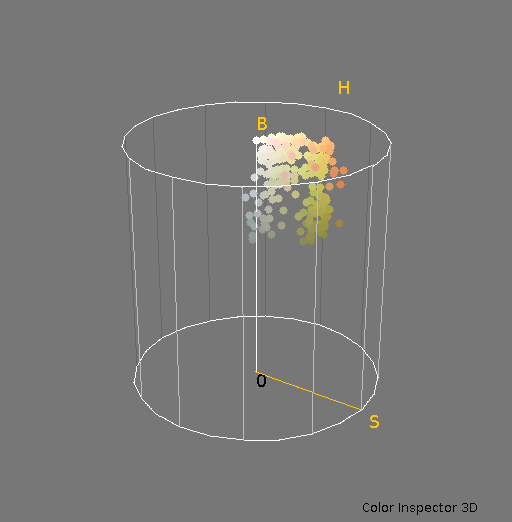
\includegraphics[width=170px]{../resultats/e1_q1_k4_lumi.png}
\end{center}
\caption{Visualisation des 2 images dans l'espace HSB}
\end{figure}

TODO expliquer différence estimée

\clearpage
\subsection{Résultats}

\subsubsection{Cas 1}

\begin{figure}[H]
\begin{center}
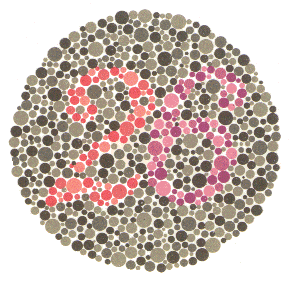
\includegraphics[width=170px]{../base/cas_1_dalton26.png}
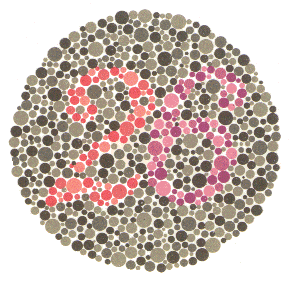
\includegraphics[width=170px]{../resultats/e1_q2_k1_luminance.png}
\end{center}
\caption{À gauche, image originale. À droite, image retouchée}
\end{figure}

TODO analyse des images

\begin{figure}[H]
\begin{center}
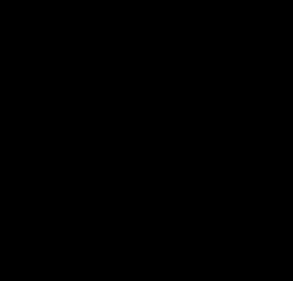
\includegraphics[width=170px]{../resultats/e1_q2_k1_diff.png}
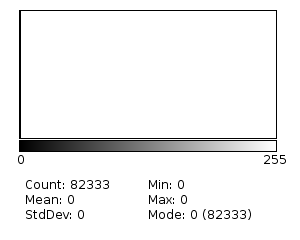
\includegraphics[width=170px]{../resultats/e1_q2_k1_diff_hist.png}
\end{center}
\caption{Carte des différences et son histogramme}
\end{figure}

\clearpage
\subsubsection{Cas 2}

\begin{figure}[H]
\begin{center}
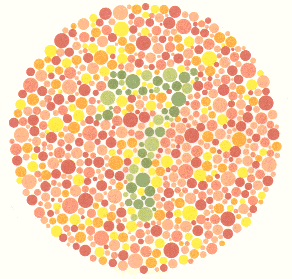
\includegraphics[width=170px]{../base/cas_2_dalton7.png}
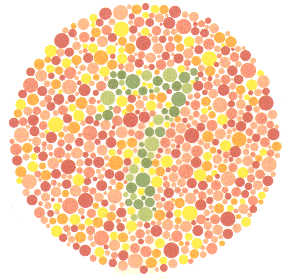
\includegraphics[width=170px]{../resultats/e1_q2_k2_luminance.png}
\end{center}
\caption{À gauche, image originale. À droite, image retouchée}
\end{figure}

TODO analyse des images

\begin{figure}[H]
\begin{center}

\includegraphics[width=170px]{../resultats/e1_q2_k2_diff.png}
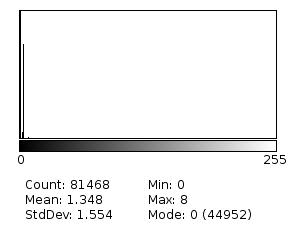
\includegraphics[width=170px]{../resultats/e1_q2_k2_diff_hist.png}
\end{center}
\caption{Carte des différences et son histogramme}
\end{figure}

\clearpage
\subsubsection{Cas 3}

\begin{figure}[H]
\begin{center}
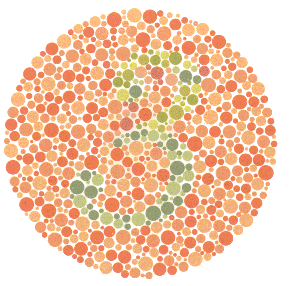
\includegraphics[width=170px]{../base/cas_3_dalton3.png}
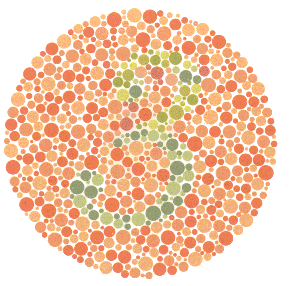
\includegraphics[width=170px]{../resultats/e1_q2_k3_luminance.png}
\end{center}
\caption{À gauche, image originale. À droite, image retouchée}
\end{figure}

TODO analyse des images

\begin{figure}[H]
\begin{center}
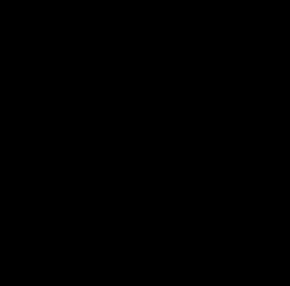
\includegraphics[width=170px]{../resultats/e1_q2_k3_diff.png}
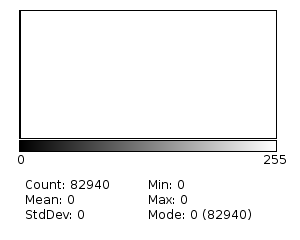
\includegraphics[width=170px]{../resultats/e1_q2_k3_diff_hist.png}
\end{center}
\caption{Carte des différences et son histogramme}
\end{figure}

\clearpage
\subsubsection{Cas 4}

TODO Pas de modification à faire


\clearpage
%----------------------------------------------------------------------------------------
% RÉTABLISSEMENT DE LA SATURATION
%----------------------------------------------------------------------------------------

\section{Rétablissement de la saturation}

\subsection{Explication}

TODO expliquer principe

\subsubsection{Cas 2}

\begin{figure}[H]
\begin{center}
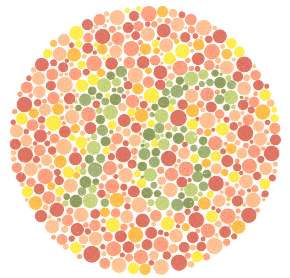
\includegraphics[width=170px]{../base/cas_2_dalton16.png}
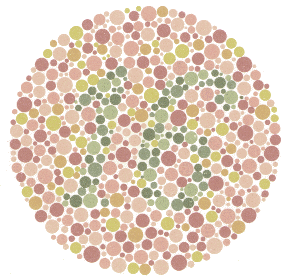
\includegraphics[width=170px]{../base/cas_2_dalton16-question2-1.png}
\end{center}
\caption{Visualisation des 2 images dans l'espace HSB}
\end{figure}

\begin{figure}[H]
\begin{center}
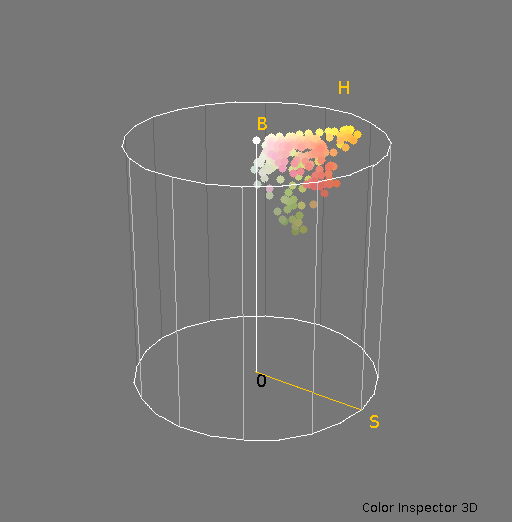
\includegraphics[width=170px]{../resultats/e2_q1_k2_16.png}
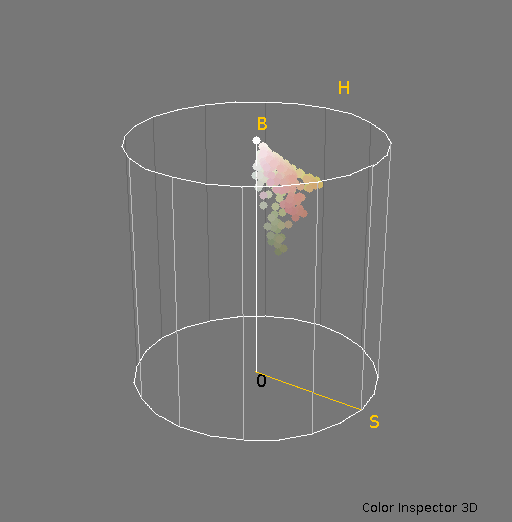
\includegraphics[width=170px]{../resultats/e2_q1_k2_modif.png}
\end{center}
\caption{Visualisation des 2 images dans l'espace HSB}
\end{figure}

TODO expliquer différence estimée

\clearpage
\subsubsection{Cas 1}

\begin{figure}[H]
\begin{center}
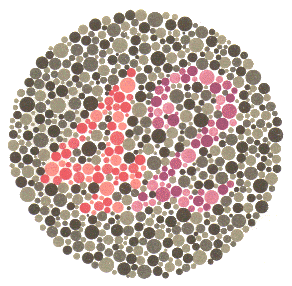
\includegraphics[width=170px]{../base/cas_1_dalton42.png}
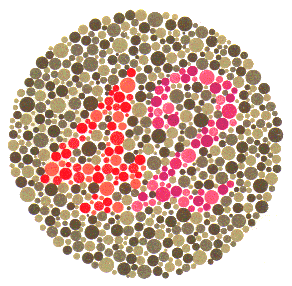
\includegraphics[width=170px]{../base/cas_1_dalton42-question2-2.png}
\end{center}
\caption{Visualisation des 2 images dans l'espace HSB}
\end{figure}

\begin{figure}[H]
\begin{center}
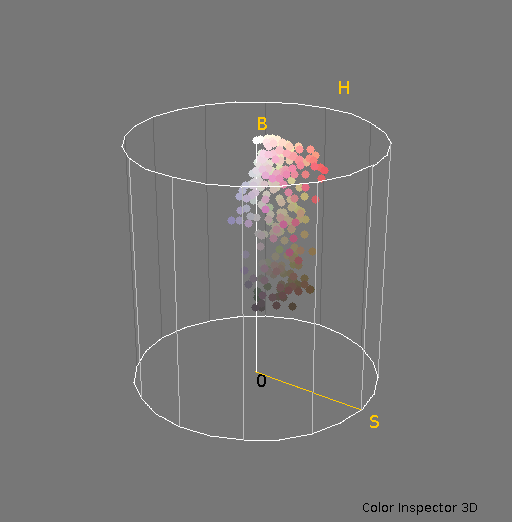
\includegraphics[width=170px]{../resultats/e2_q2_k1_42.png}
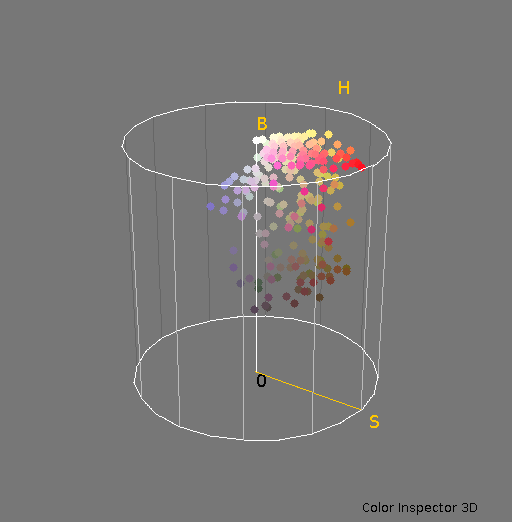
\includegraphics[width=170px]{../resultats/e2_q2_k1_modif.png}
\end{center}
\caption{Visualisation des 2 images dans l'espace HSB}
\end{figure}

TODO expliquer différence estimée

\clearpage
\subsection{Résultats}
\subsubsection{Cas 2}

\begin{figure}[H]
\begin{center}
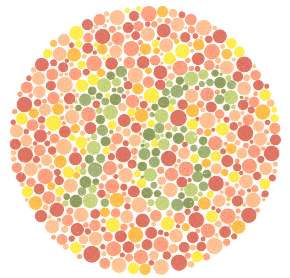
\includegraphics[width=170px]{../base/cas_2_dalton16.png}
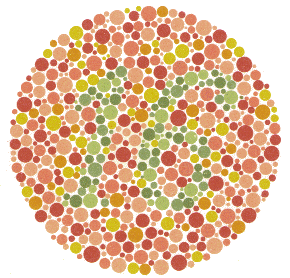
\includegraphics[width=170px]{../resultats/e2_q3_1_modif.png}
\end{center}
\caption{À gauche, image originale. À droite, image retouchée}
\end{figure}

TODO analyse résultats

\begin{figure}[H]
\begin{center}
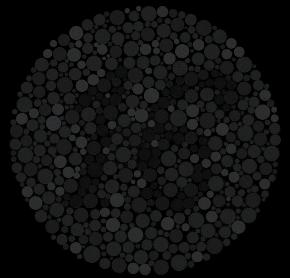
\includegraphics[width=170px]{../resultats/e2_q3_1_diff.png}
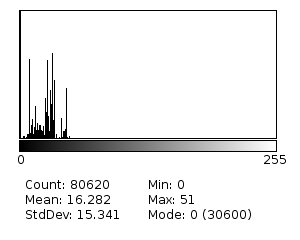
\includegraphics[width=170px]{../resultats/e2_q3_1_diff_hist.png}
\end{center}
\caption{Carte des différences et son histogramme}
\end{figure}


\clearpage
\subsubsection{Cas 1}

\begin{figure}[H]
\begin{center}
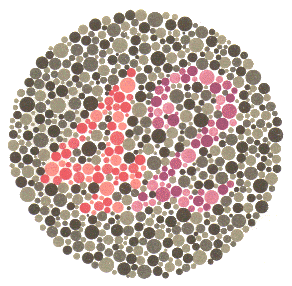
\includegraphics[width=170px]{../base/cas_1_dalton42.png}
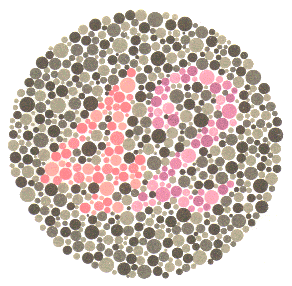
\includegraphics[width=170px]{../resultats/e2_q3_2_modif.png}
\end{center}
\caption{À gauche, image originale. À droite, image retouchée}
\end{figure}

TODO analyse résultats

\begin{figure}[H]
\begin{center}
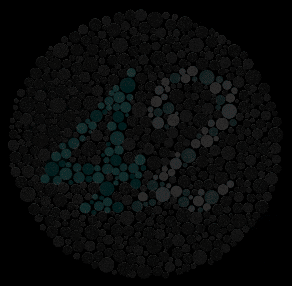
\includegraphics[width=170px]{../resultats/e2_q3_2_diff.png}
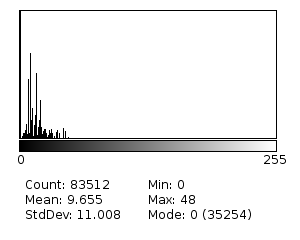
\includegraphics[width=170px]{../resultats/e2_q3_2_diff_hist.png}
\end{center}
\caption{Carte des différences et son histogramme}
\end{figure}

\clearpage
%----------------------------------------------------------------------------------------
%	TRANSFORMATION DE LA TEINTE
%----------------------------------------------------------------------------------------

\section{Transformation de la teinte}

\subsection{Explication}

TODO expliquer principe

\subsubsection{Cas 3}

\begin{figure}[H]
\begin{center}
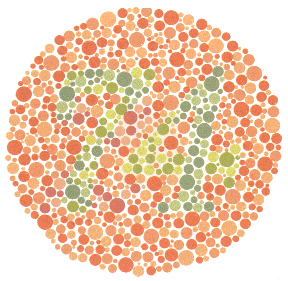
\includegraphics[width=170px]{../base/cas_3_dalton74.png}
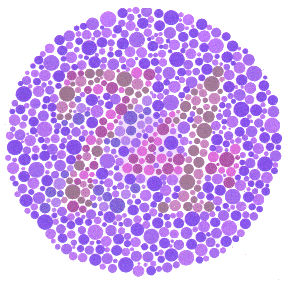
\includegraphics[width=170px]{../base/cas_3_dalton74_question3_1.png}
\end{center}
\caption{À gauche, image originale. À droite, image modifiée}
\end{figure}

\begin{figure}[H]
\begin{center}
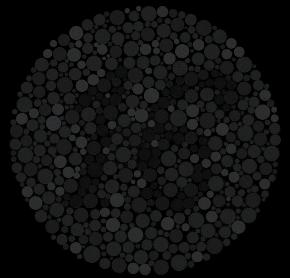
\includegraphics[width=170px]{../resultats/e2_q3_1_diff.png}
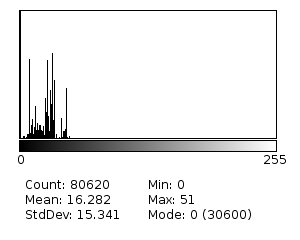
\includegraphics[width=170px]{../resultats/e2_q3_1_diff_hist.png}
\end{center}
\caption{Visualisation des 2 images dans l'espace HSB}
\end{figure}

TODO expliquer différence estimée

\clearpage
\subsection{Résultats}
\subsubsection{Cas 3}

\begin{figure}[H]
\begin{center}
\includegraphics[width=170px]{../base/cas_3_dalton74.png}
\includegraphics[width=170px]{../resultats/e3_q1_modif.png}
\end{center}
\caption{À gauche, image originale. À droite, image retouchée}
\end{figure}

TODO analyse résultats

\begin{figure}[H]
\begin{center}
\includegraphics[width=170px]{../resultats/e3_q1_diff.png}
\includegraphics[width=170px]{../resultats/e3_q1_diff_hist.png}
\end{center}
\caption{Carte des différences et son histogramme}
\end{figure}

\clearpage

%----------------------------------------------------------------------------------------
%	ANALYSE DANS DES ESPACES COULEURS ADAPTÉS
%----------------------------------------------------------------------------------------

\section{Analyse dans des espaces couleur adaptés}

\subsection{Explication}

TODO expliquer question

\subsubsection{Cas 3}

\begin{figure}[H]
\begin{center}
\includegraphics[width=170px]{../base/cas_3_dalton74.png}
\includegraphics[width=170px]{../base/cas3_dalton74_question4_1.png}
\end{center}
\caption{À gauche, image originale. À droite, image modifiée}
\end{figure}

\begin{figure}[H]
\begin{center}
\includegraphics[width=170px]{../resultats/e4_visu_original.png}
\includegraphics[width=170px]{../resultats/e4_visu_modif.png}
\end{center}
\caption{Visualisation des 2 images dans l'espace HSB}
\end{figure}

\clearpage
\subsection{Analyse}

TODO analyse

\clearpage
%----------------------------------------------------------------------------------------
%	MODIFICATION DE LA LUMINANCE ADAPTÉE
%----------------------------------------------------------------------------------------

\section{Modification de la luminance adaptée}

\subsection{Explication}

TODO expliquer question

\subsubsection{Cas 1}

\begin{figure}[H]
\begin{center}
\includegraphics[width=170px]{../base/cas_1_dalton42.png}
\includegraphics[width=170px]{../base/cas_1_dalton42-question5.png}
\end{center}
\caption{À gauche, image originale. À droite, image modifiée}
\end{figure}

\begin{figure}[H]
\begin{center}
\includegraphics[width=170px]{../resultats/e5_visu_original.png}
\includegraphics[width=170px]{../resultats/e5_visu_modif.png}
\end{center}
\caption{Visualisation des 2 images dans l'espace HSB}
\end{figure}

\clearpage
\subsection{Analyse}

TODO analyse

\clearpage
%----------------------------------------------------------------------------------------

%----------------------------------------------------------------------------------------
%	CONCLUSION
%----------------------------------------------------------------------------------------

\section{Conclusion}
Nous avons pu constater qu'une image possède plusieurs composantes, mais que celles-ci peuvent différer en fonction de la représentation de l'image, ou espace colorimétrique.\\

Chaque opération sur un espace colorimétrique aura un effet propre à l'espace. De plus, les jeux de composantes pourront mettre en évidence différents phénomènes apparaissant sur l'image.\\
Il existe cependant une limite aux opérations sur les espaces colorimétriques. Lorsqu'une image a été modifiée, il est possible de perdre de l'information à cause d'un effet de plancher/plafond.\\

Il peut donc être utile de convertir un espace colorimétrique en un autre afin de pouvoir profiter d'opérations spécifiques, ou pour analyser la composition de l'image sous un autre angle.

\clearpage
%----------------------------------------------------------------------------------------

\section{Annexe}

\subsection{Manipulation de la luminance}
\lstinputlisting{../add_brightness.ijm}
TODO reproprer code

\subsection{Rétablissement de la saturation}
\lstinputlisting{../mul_saturation.ijm}
TODO reproprer code

\subsection{Transformation de la teinte}
\lstinputlisting{../change_hue.ijm}
TODO reproprer code

\end{document}
